
%(BEGIN_QUESTION)
% Copyright 2015, Tony R. Kuphaldt, released under the Creative Commons Attribution License (v 1.0)
% This means you may do almost anything with this work of mine, so long as you give me proper credit

\noindent

\vskip 5pt

\begin{center}
\vskip 5pt 
\textbf{Målesystemer -- Nivå 2 }
\vskip 5pt 
\textbf{Arbidsoppdrag på Stasjon 15}
\vskip 5pt 
\textbf{Digitale målesystemer}
\end{center}

\textbf{Introduksjon}

I denne oppgaven skal du koble opp og teste ulike digitale målesystemer



\begin{enumerate}
\item Mekanisk endebryter med rulle
\item Mekanisk endebryter med fjær
\item Mekanisk endebryter med aksling....
\item kapasitiv nærhetssensor 
\item induktiv nærhetssensor
\item Photo sensor 
\end{enumerate}


$$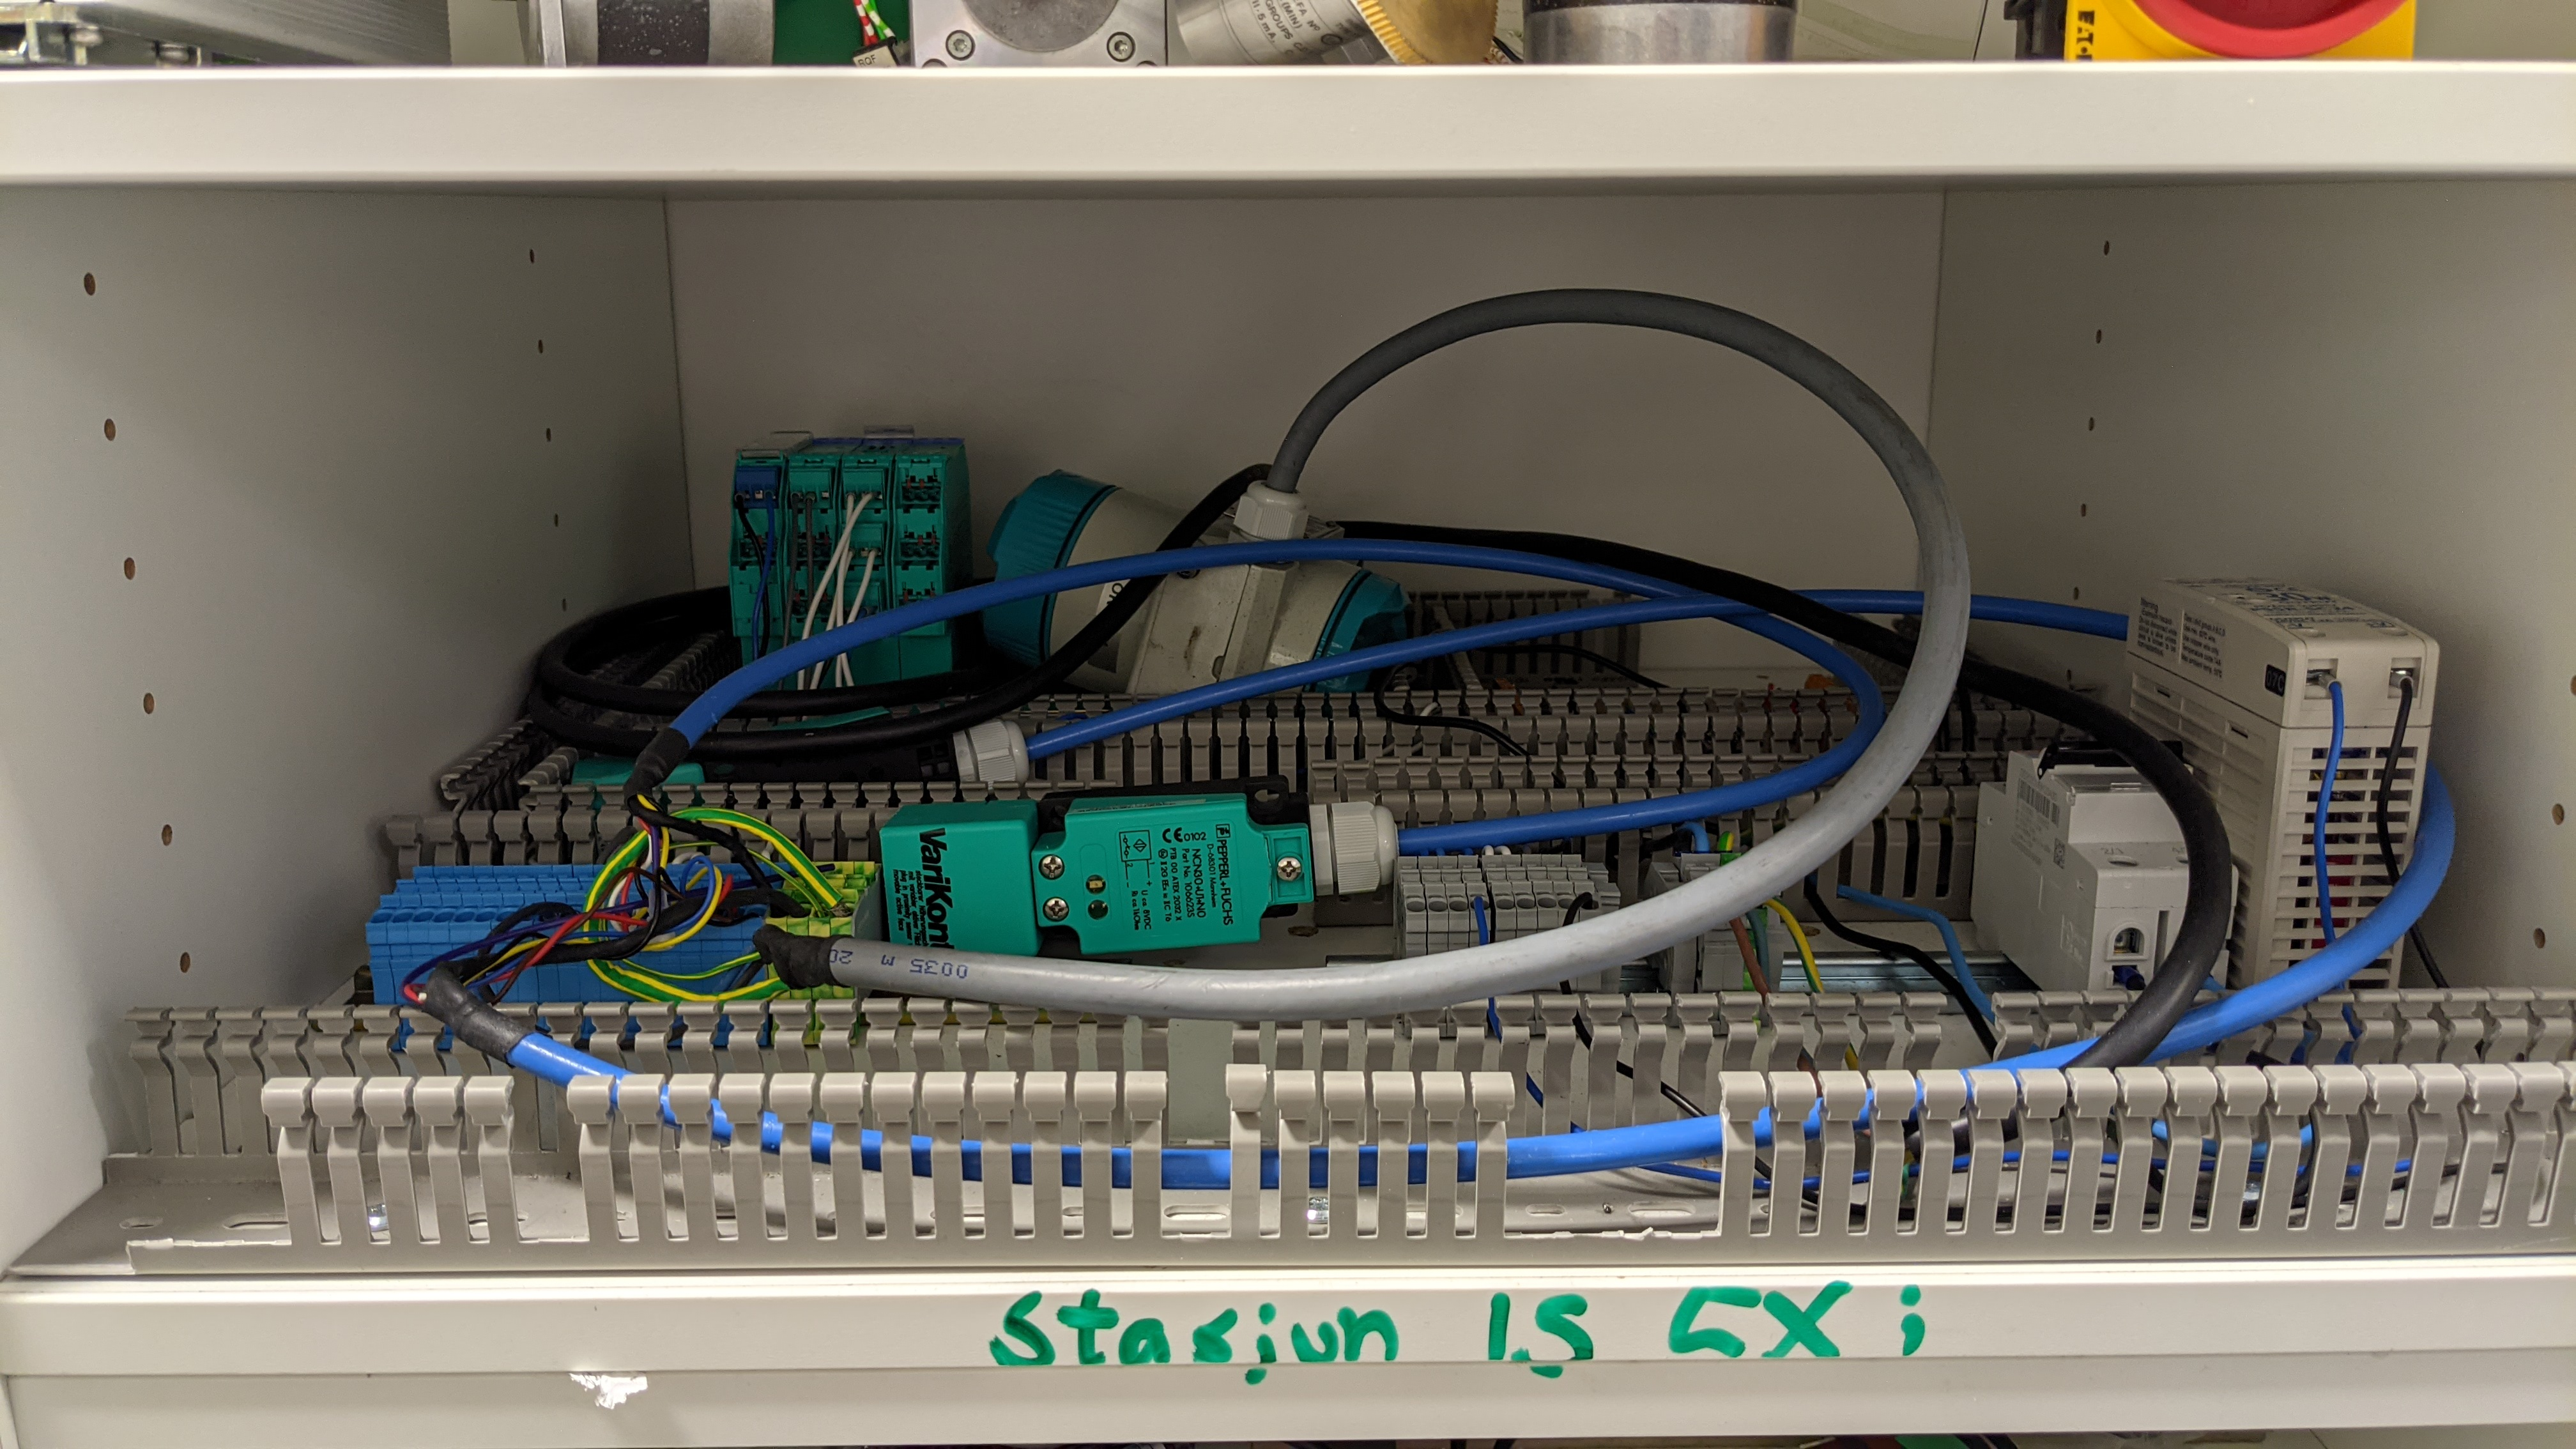
\includegraphics[width=10.5cm]{stasjon15x01.jpg}$$
\textbf{Teorioppgaver}

\vskip 5pt 
Her er noen tekster der du kan lese deg opp på endebrytere

\vskip 5pt 
\href{https://www.eaton.com/ecm/groups/public/@pub/@electrical/documents/content/pct_1549250.pdf}{The Basics of Limit Switches - Eaton guide til endebrytere}
\vskip 5pt 
\href{https://www.edata.omron.com.au/eData/Switches/X019-E1-07.pdf}{Omron komplett katalog}
\vskip 5pt 
\href{https://www.ia.omron.com/data_pdf/guide/30/limitswitch_apparatus_tg_e_3_2.pdf}{Omron guide til limit switches}
\vskip 5pt 
\href{https://stevenengineering.com/tech_support/PDFs/45LS.pdf}{ukjent}
\vskip 5pt 
\textbf{Planlegging}

\textbf{Gjennomføring}

\textbf{Dokumentasjon}

\vskip 5pt
\begin{center}
\textbf{Arbidsoppdrag}
\vskip 5pt 
\textbf{Programmering av reguleringsstasjon}
\end{center}

\vskip 10pt 
\textbf{Introdusjon}

\vskip 5pt 

\vskip 5pt 

%$$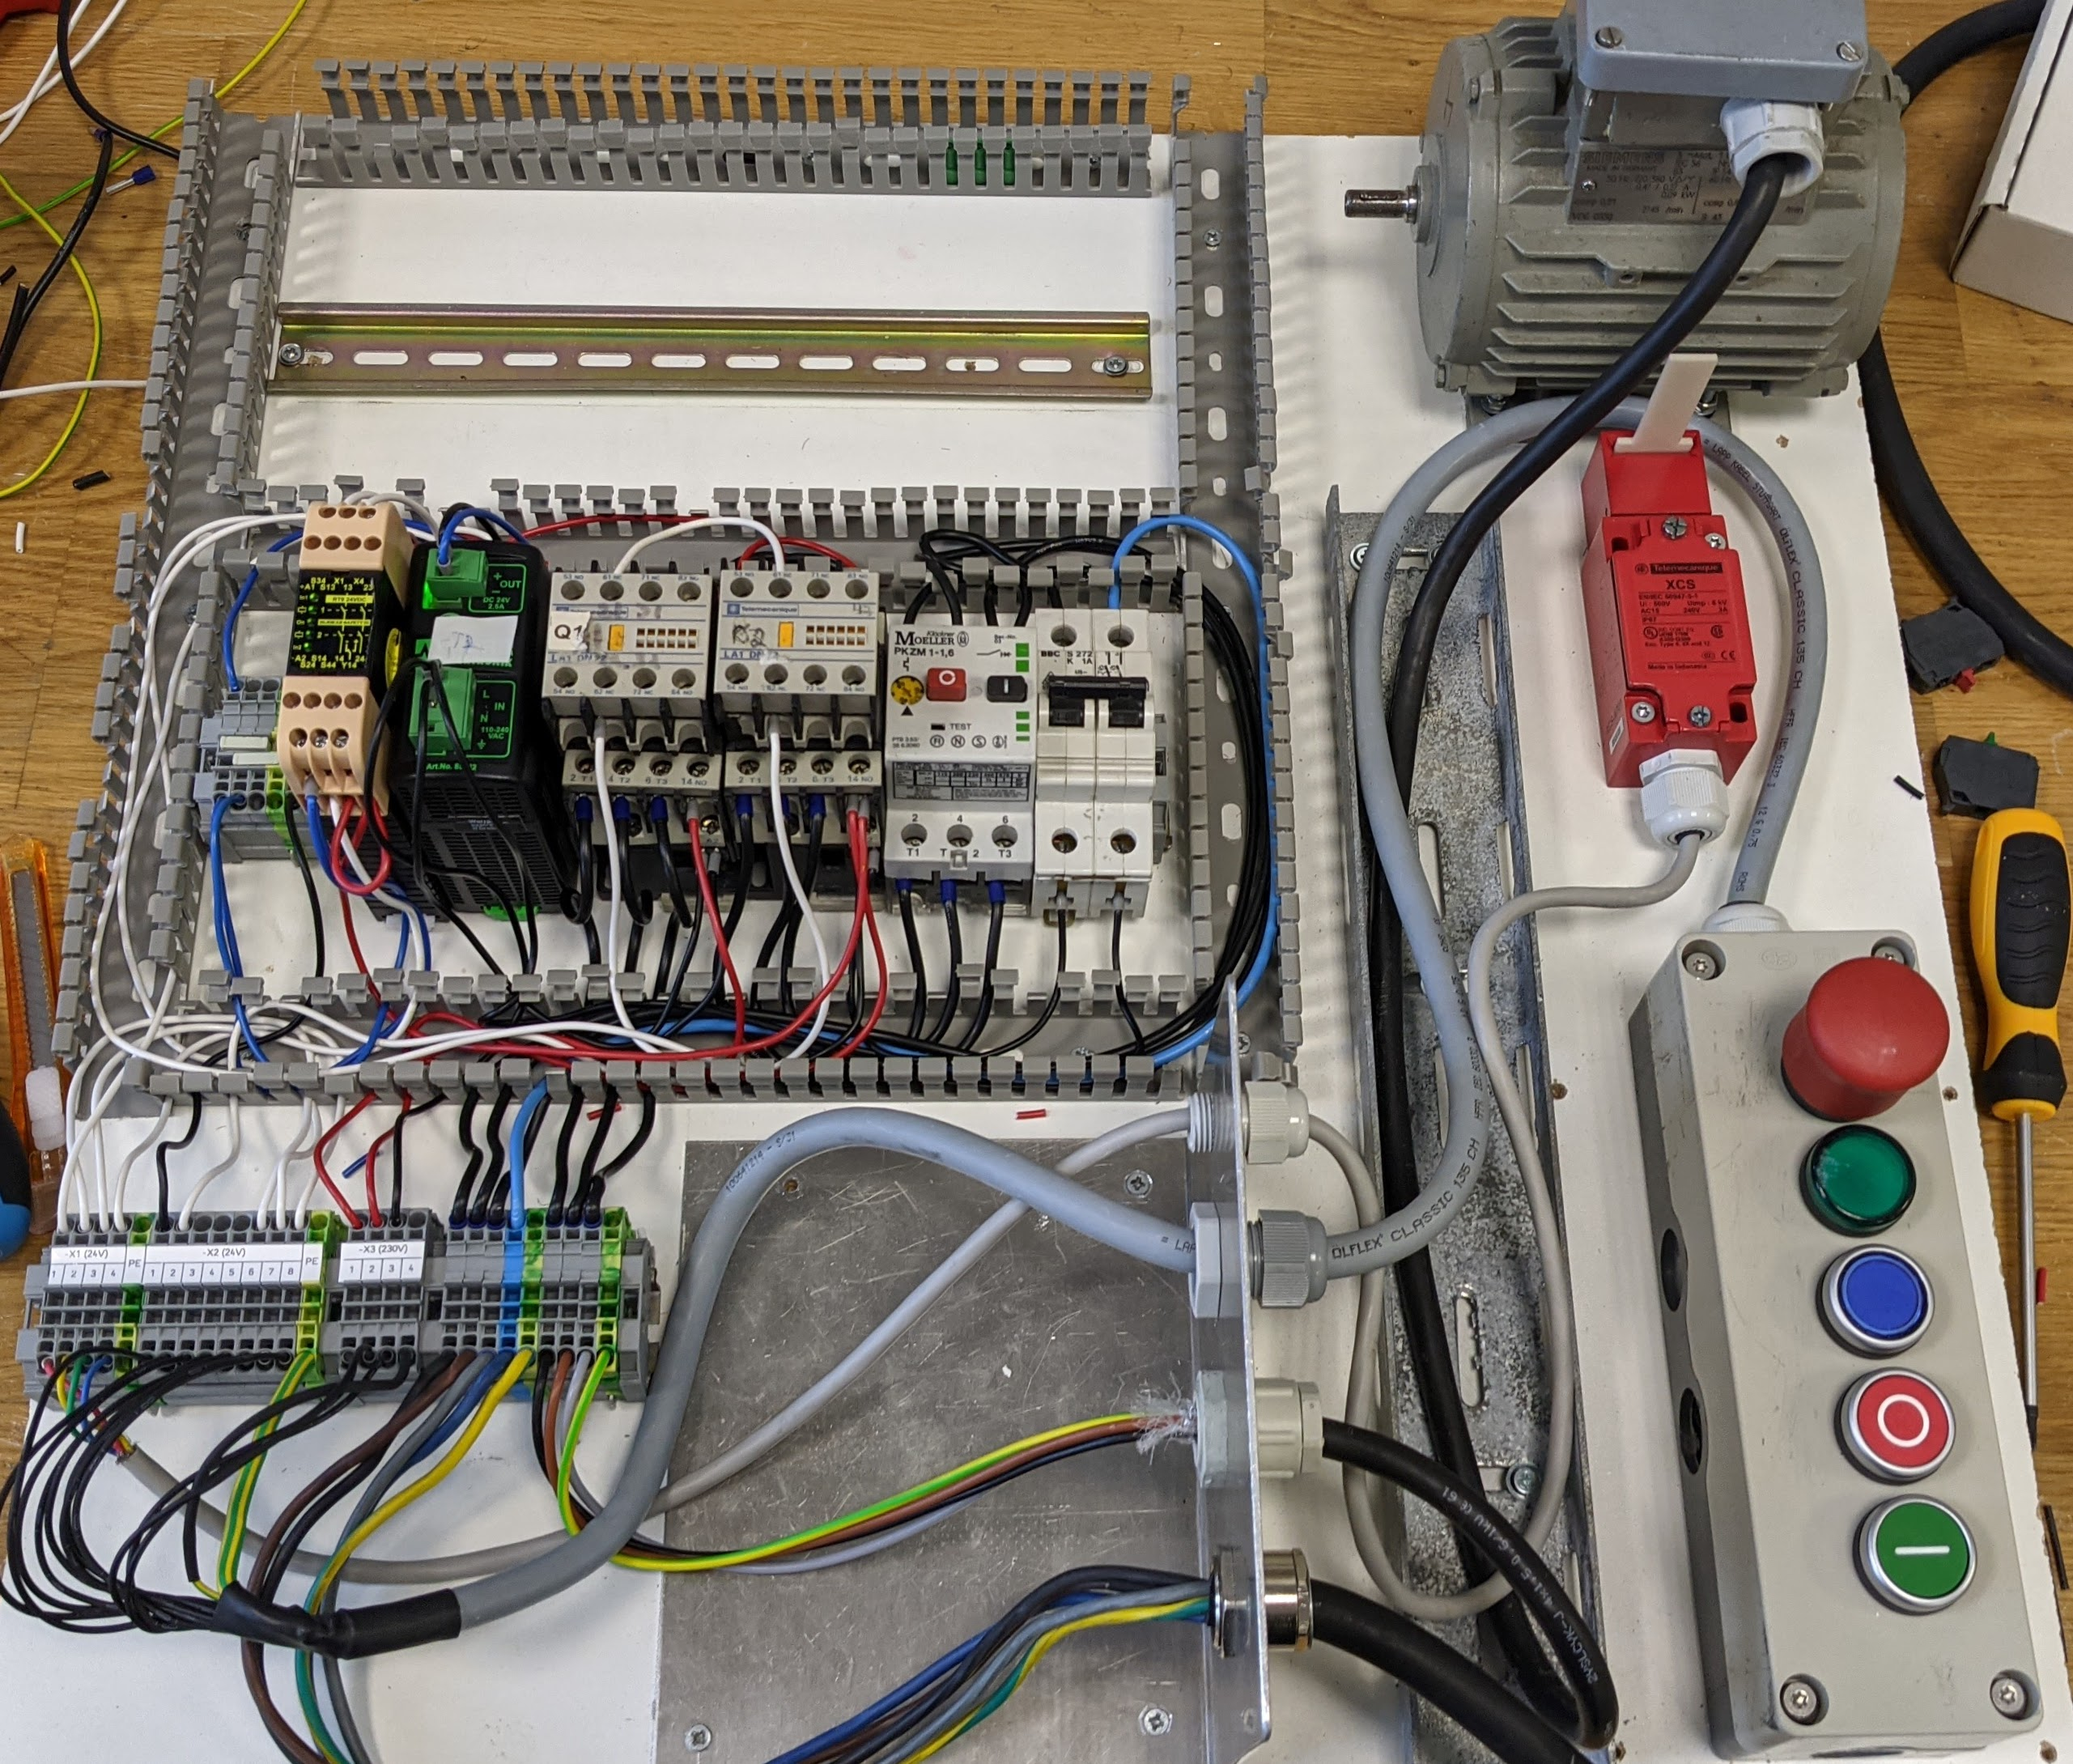
\includegraphics[width=13cm]{i04821x01.jpg}$$\\

\vskip 10pt 
\textbf{Teorioppgaver}

\vskip 5pt 

\vskip 10pt 
\textbf{Planlegging}


\vskip 10pt 
\textbf{Gjennomføring}

\vskip 10pt 
\textbf{Dokumentasjon}

Beskriv hvordan du planlegger, gjennomfører og dokumenterer denne jobben. 





















\underbar{file i04844}
\vfil \eject
%(END_QUESTION)





%(BEGIN_ANSWER)


%(END_ANSWER)





%(BEGIN_NOTES)


%INDEX% Arbeisdoppdrag, Kompetanse, Nivå 1, Stasjonxx, Mal

%(END_NOTES)


